\newpage
\nnchapter{Apéndices}
% ------------------------------------------------------------------------
\anexo{Simulación de las interacciones electromagnéticas y hadrónicas en CORSIKA}\label{sec:apendiceA}

\noindent\textbf{1. Interacciones electromagn\'eticas}

CORSIKA proporciona dos rutinas diferentes para el análisis de las interacciones electromagnéticas de la EAS: FNKG que calcula de forma analítica las subcascadas electromagnéticas usando la información suministrada por el usuario del tipo de primario y los límites en energía. Y EGS4, que es una rutina Monte Carlo para calcular las interacciones de forma explícita a partir de distribuciones estadísticas. Para este trabajo, se utilizó la rutina EGS4 de la cual explicaremos algunas de sus consideraciones físicas más importantes.\\

EGS4 es un programa analógico de Monte Carlo, es decir, todas y cada una de las partículas son seguidas hasta su destino final hasta algún límite inferior de energía. En concordancia con la naturaleza de el método estadístico de Monte Carlo, la precisión de los resultados dependerá del número de eventos analizados. Generalmente, las incertidumbres estadísticas son proporcionales a la raíz inversa del número de eventos\citep{EGS4}. También para una energía mínima dada, el tiempo de cómputo para una lluvia de alta energía es alto. Por esta razón que EGS4 está dividido en dos partes, la primera, un código procesador que usa fórmulas teóricas y empíricas para calcular las cantidades físicas que se necesitan y las prepara para realizar una evaluación numérica rápida. Estos datos son los que usa para desarrollar toda la simulación \citep{EGS4}.\\

EGS4 considera los siguientes procesos:

\begin{itemize}
    \item Radiación de frenado o Bremsstrahlung
    \item Aniquilación de positrones
    \item Dispersión múltiple de Coulomb
    \item Dispersión de Moller ($e^{-}e^{-}$) y Bhabha ($e^{-}e^{+}$)
    \item Pérdida continua de energía
    \item Producción de pares
    \item Dispersión Compton
    \item Dispersión de Rayleight (opcional)
    \item Efecto fotoeléctrico
\end{itemize}{}

Los procedimientos Monte Carlo cambian respecto al tipo de partícula y tipo de interacción. Por ejemplo, para los fotones, la distancia al siguiente punto de interacción, se obtiene por una distribución exponencial que se establece a partir del coeficiente de atenuación, y el tipo de interacción es determinado a través del cálculo de probabilidades relativas. Para los electrones, las interacciones elásticas e inelásticas de Coulomb son difíciles de calcular directamente, de esta forma, EGS4 divide las trayectorias del electrón en muchos segmentos en los cuales ocurren numerosas interacciones y, para cada segmento, la deflexión angular y la pérdida de energía, son calculadas a partir de distribuciones de dispersión múltiple \citep{EGS4book}.  \\

En el proceso de propagación de las partículas cargadas en el aire, estas pierden energía por ionización. Mientras que las partículas neutras continúan su camino sin pérdidas. Debido a la gran capacidad de penetración de de los $\mu\pm $, se tiene en cuenta con ellas el fenómeno de dispersión múltiple de Coulomb. Además, todas las trayectorias de partículas cargadas son curvadas por el campo magnético terrestre. Finalmente, si las partículas pasan un nivel de observación mientras están siendo seguidas  hasta el siguiente punto de interacción, sus coordenadas de espacio, momento y tiempo son almacenadas. Veamos cómo EGS4 considera algunos de estos procesos:\\

\textbf{Pérdida de energía por Ionización}: La pérdida de energía por ionización de una partícula cargada que atraviesa la materia con un espesor $\lambda$ es descrita por la ecuación de Bethe-Bloch:

\begin{equation*}
dE_{i} =  \frac{\lambda z^{2}}{\beta^{2}}\kappa_{1}(ln(\gamma^{2}-1)- \beta^{2}+\kappa_{2})
\end{equation*}
%
\begin{equation}
dE_{i} = \frac{\lambda \gamma^{2}z^{2}}{\gamma^{2}-1}\kappa_{1}(ln(\gamma^{2}-1)- \beta^{2}+\kappa_{2})
\label{eq:eq20}
\end{equation}

Donde $\beta = v/c $ es la velocidad de la partícula en unidades de la velocidad de la luz, $\gamma$ es el factor de Lorentz, $z$ es la carga de la partícula ionizada en unidades de $e$. Las dos constantes $\kappa_{1}= 0.153287 MeV g^{-1}$ y $\kappa_{2}= 9.386417 MeV g^{-1}$ son los valores correspondientes para el aire \citep{Heck1998}. Esta expresión es usada para calcular la perdida por energía de ionización a través de la trayectoria de la partícula. La pérdida de energía de muones como función de su energía está representado en la figura \ref{fig:fig4}.\\

\begin{figure}[htb!]
        \begin{center}
        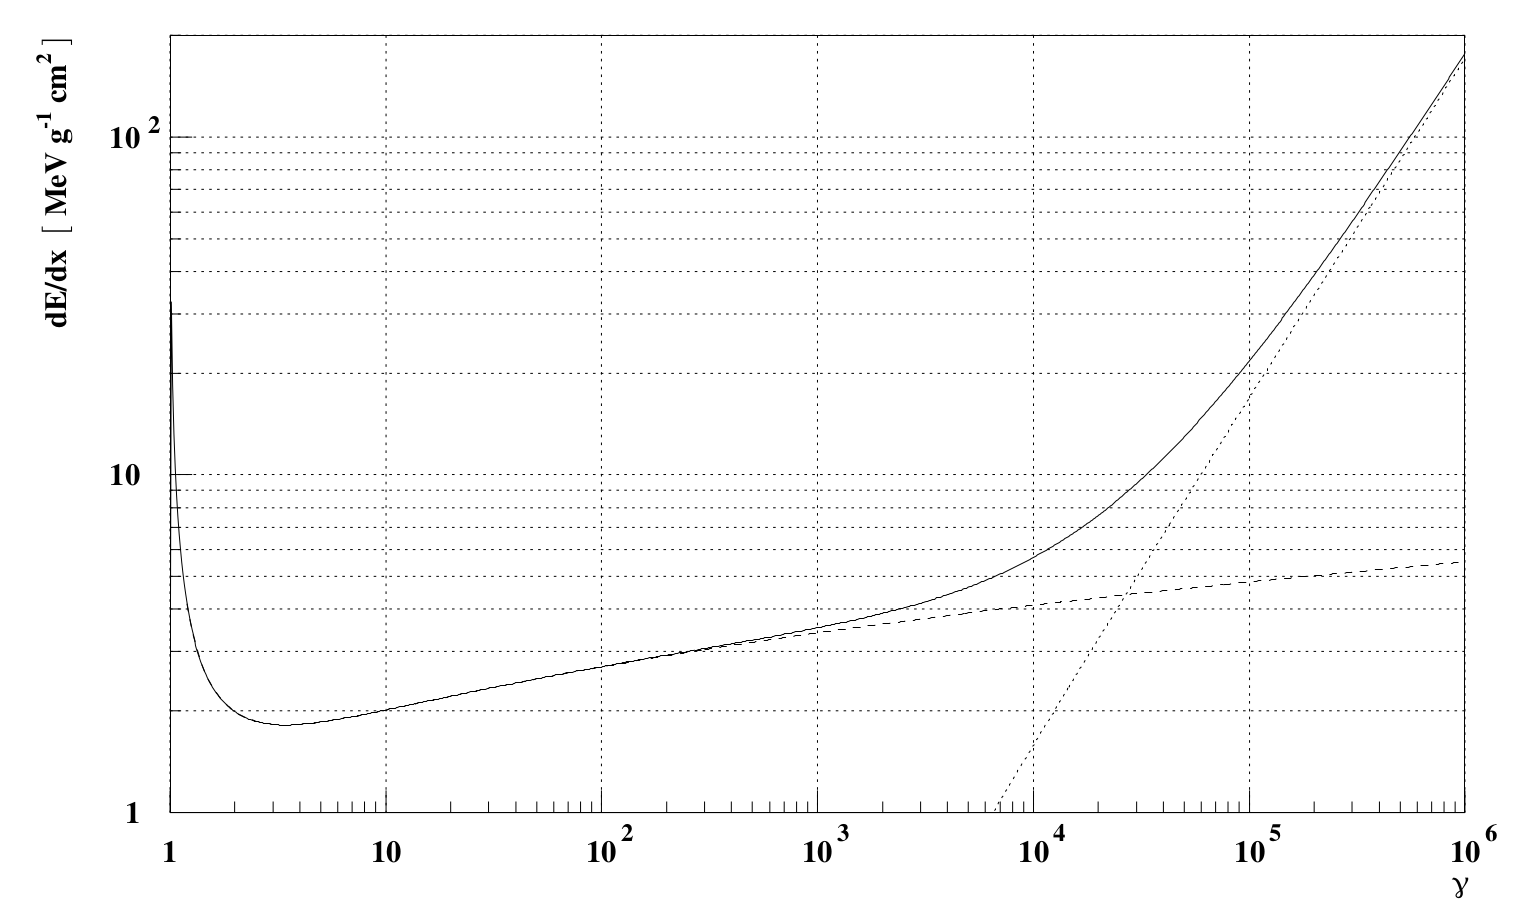
\includegraphics[width=1\textwidth]{Figs/Bethe_Muons.png}
        \end{center}
        \caption[Ecuación de Bethe-Bloch para los muones.]{Pérdida de energía de Muones en el aire como función del factor de Lorentz \citep{Heck1998}. Están indicadas las contribuciones de la ionización (línea seccionada) y la producción de pares (línea punteada).}
        \label{fig:fig4}
\end{figure}

\textbf{Dispersión múltiple de Coulomb}: Las partículas cargadas son dispersadas por el campo eléctrico Coulombiano de los núcleos de aire, en esta situación, la dirección de propagación es alterada pero no cambia la energía de la partícula. En CORSIKA el proceso de dispersión múltiple es considerado sólo en muones y solo una vez por cada tramo de trayectoria. La distribución angular de esta dispersión es descrita por la teoría de Moliére. Es importante destacar que, para partículas de altas energías, esta dispersión no es relevante. En la dispersión de Moliere, la determinación del ángulo de dispersión, se rige por el número de dispersiones a través de un espesor $\lambda$ de acuerdo con:

\begin{equation}
\centering
\Omega_{0} = 6702.33 \frac{\lambda}{\beta^{2}} \frac{Z_{s}}{m_{air}}e^{Z_{e}-Z_{x} /Z_{x}}
\label{eq:eq21}
\end{equation}

donde $\beta$ es la velocidad del muon en unidades de la velocidad de la luz y $m_{air} = 14.54$ es el promedio del peso atómico del aire. Las cantidades $Z_{s}$, $Z_{e}$ y $Z_{x}$ dependen de las fracciones atómicas $n_{i}$ de los átomos del tipo $i$ con carga número $Z_{i}$ en el aire. Si el número eventos dispersivos es bajo (menores a 20), el ángulo total de dispersión se toma como la suma geométrica de las dispersiones individuales, si no, es modelado por:

\begin{equation}
\centering
f(\theta) \theta d\theta = \sqrt{\frac{sin\theta}{\theta}} f_{r}(\eta) d \eta
\label{eq:eq22}
\end{equation}

\textbf{Deflexión causada por el campo magnético de la Tierra}:  El campo magnético de la tierra es caracterizado por la fuerza $B_{E}$, el ángulo de declinación $\delta$ y el ángulo de inclinación $\theta$. \\

Una partícula de carga $Z$ y momento $\Vec{p}$ moviéndose a través de la longitud de su trayectoria $l$ en un campo magnético $\Vec{B}$, experimenta una deflexión que apunta a la dirección normal del plano atravesado por $\Vec{B}$ y $p$. Para ángulos pequeños esta dada por:

\begin{equation}
\centering
\alpha \approx lZ \frac{\Vec{p} \times \Vec{B}}{p^{2}}
\label{eq:eq23}
\end{equation}

\textbf{Tiempo de vuelo}: Después de la primera interacción del primario con la atmósfera, el tiempo de la lluvia comienza. EL intervalo de tiempo $dt$ en el cual una partícula se mueve alrededor de su trayectoria se obtiene dividiendo la longitud recorrida por la velocidad promedio de la partícula como,

\begin{equation}
\centering
dt = \frac{l}{c\beta_{prom}}
\label{eq:eq24}
\end{equation}

y el tiempo total que transcurre desde la primera interacción es la suma de los intervalos acumulados por las sucesivas partículas hasta un nivel de observación definido.\\

\noindent\textbf{2. Interacciones hadr\'onicas}

Los canales de interacción electromagnética y electrodébil dentro del modelo estándar de la física de partículas, describen muy bien los procesos involucrados en las EAS. Sin embargo, el limitado conocimiento de las interacciones fuertes llega a ser una fuente dominante de indeterminación en los procesos de las lluvias. Aunque la cromodinámica cuántica (QCD) es una teoría de interacción fuerte bien establecida y confirmada experimentalmente, sólo los procesos con gran transferencia de momento pueden ser predichos en base a principios fundamentales hasta ahora \citep{Allen}. \\

Como no es posible calcular las  propiedades de la producción de múltiples partículas en las interacciones hadrónicas de manera precisa, para analizar las EAS, se construyen modelos que realizan supuestos adicionales, parametrizaciones fenomenológicas y empíricas, que complementen la falta de información. Luego de creados los modelos, son verificados y restringidos a partir de los datos obtenidos de aceleradores. Los modelos construidos para la interpretación de las EAS, deben estar optimizados para un rango de energías amplio, y deben ser constantemente actualizados, conforme se obtienen más datos en los aceleradores.\\

En CORSIKA, las interacciones hadrónicas son simuladas mediante diferentes modelos dependiendo de la energía. A bajas energías, usa el modelo GHEISHA o ISOBAR. Si la energía es lo suficientemente grande, la interacción es tratada con alguno de los modelos: VENUS, QGSJET, DPMJET, SIBYLL o HDPM. Los modelos de altas energías  alcanzan su límite si la energía de centro de masa disponible está por debajo de  un umbral, $12 GeV$ para la transición de GHEISHA. \\

Las rutinas GHEISHA tratan a los neutrones de baja energía de una manera muy consistente. Comparándola con la rutina ISOBAR, donde los neutrones de baja energía son dispersados alrededor de una pérdida de energía de una forma poco realista \citep{Allen}, resultando en numerosos neutrones de baja energía. Por tal razón, CORSIKA recomienda siempre el uso de GHEISHA a pesar de aumentar el tiempo de cómputo con ello.\\

\textbf{Interacciones fuertes a altas energías}: La figura muestra una comparación entre los códigos disponibles en CORSIKA y datos obtenidos del CMS el flujo de energía como función de la pseudorapidez en dirección del movimiento de la partícula. Además, los datos de los modelos han sido contrastados con las simulaciones realizadas para el CMS. Para este trabajo, se usará el modelo QGSJET-II.\\
%en el colisionador proton-antiproton del CERN \citep{Alner1986}, a partir de la distribución de pseudorapidez para una energía de centro de masa $E_{cm} = 200 GeV$
\begin{figure}[htb!]
\centering
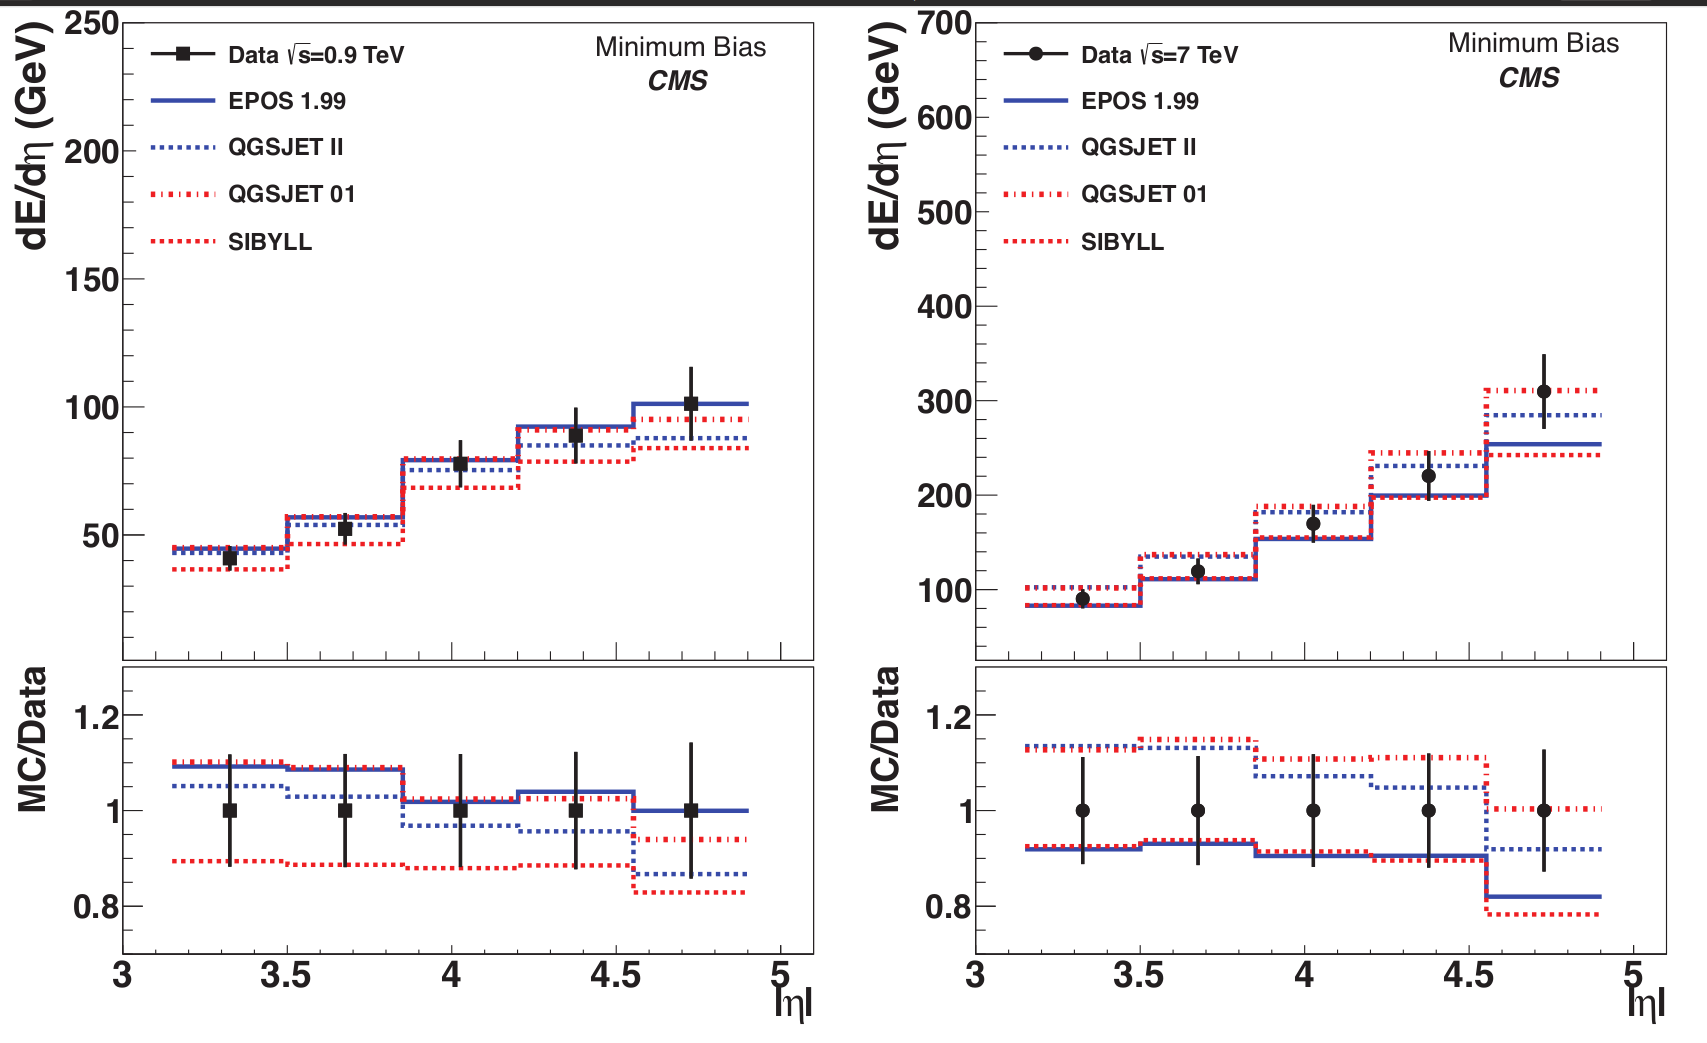
\includegraphics[width=1\textwidth]{Figs/Hadronic_Model_Comparison_3.png}
\caption[Flujo de energía para hadrones de alta energía]{Gráfica del flujo de energía como función de la pseudorapidez en la dirección del movimiento de hadrones con energía de centro de masa de 900GeV. \citep{Allen} }
        \label{fig:fig5}
\end{figure}

\newpage